% vim: spell spelllang=en_us
\documentclass[conference,12pt]{IEEEtran}
\usepackage[T1]{fontenc}
\usepackage[utf8]{inputenc}
\usepackage[english]{babel}
\usepackage{csquotes}
\usepackage{biblatex}
\usepackage{amsmath}
\usepackage{minted}
\usepackage[inline]{enumitem}
\usepackage{amsthm}
\usepackage{mdframed}
\usepackage{graphicx}
\usepackage{subcaption}

\MakeOuterQuote{"}

\addbibresource{references.bib}

\setminted{autogobble,python3,mathescape,frame=lines,framesep=2mm,fontsize=\footnotesize,escapeinside=~~}
\newcommand\tab[1][.5in]{\hspace*{#1}}
\newcommand\name{VRsh}
\newtheorem{definition}{Definition}

\title{Final Project Report}
\author{%
    \IEEEauthorblockN{%
        Jonathan Sumner Evans\IEEEauthorrefmark{1},
        Robinson Merillat\IEEEauthorrefmark{2}, and
        Sam Sartor\IEEEauthorrefmark{3}
    }
    \IEEEauthorblockA{%
        Department of Computer Science,
        Colorado School of Mines\\
        Golden, Colorado\\
        Email:
            \IEEEauthorrefmark{1}jonathanevans@mines.edu,
            \IEEEauthorrefmark{2}rdmerillat@mines.edu,
            \IEEEauthorrefmark{3}ssartor@mines.edu
    }
}

\begin{document}
\maketitle
\begin{abstract}
    Virtual Reality (VR) Technology has been developing rapidly over the past
    decade. Current solutions such as Unity attempt to use old programming
    languages and even older paradigms to implement VR applications and thus,
    limit developers' abilities to create new and unique environments.  With
    every cutting edge technology, new paradigms and design patterns must be
    invented.  In this paper, we discuss a deferred immediate mode (DIM)
    application architecture suitable for implementing large virtual reality
    applications.  We present a UI library which utilizes this architecture and
    a few case studies of this library in use.
\end{abstract}

\section{Introduction}\label{sec:introduction}

The Virtual Reality (VR) market is growing rapidly. The International Data
Corporation (IDC) projects that revenues for the combined Augmented Reality (AR)
and Virtual Reality markets will grow from \$5.2 billion in 2016 to more than
\$162 billion in 2020~\cite{IDC:2016:VR-industry}. This flourishing new industry
has created an exciting new field of Software Engineering with great potential
for revolutionary new design paradigms and program architectures.

Most current frameworks and libraries attempt to apply old design paradigms and
program architectures to virtual reality. While these paradigms and
architectures are well-suited for 2D user interfaces and rendering 3D
environments to a flat screen, they are not designed with VR in mind. Although
endeavors to adapt these old patterns to VR have been successful, they are
restrictive in both the code architecture and way of thinking. Grace Hopper
loved to say "The most damaging phrase in the language is: `It's always been
done that way'"~\cite{Hopper:1987:quote}. This quote promotes new ways of
thinking. Utilizing outdated architectures hinders the exploration and the
potential for new design paradigms and program architectures.

Our goal is to find a system that provides a modern, fast, and practical
approach to virtual reality development. Specifically, we require that this
system meets the following criteria.

\subsection{Performant}\label{sec:performant}

Traditionally, animation is done at approximately 60 frames per second.  This is due to
the dominance of monitors and televisions that ran at 60Hz and had a refresh rate of
60 frames per second (fps).  This frame rate is acceptable when viewing a screen from a
distance. However, in order to appear believable and prevent disorientation, a
virtual reality program must run at at least 90 fps. In fact, many studies have
shown that when VR is run with lower frame rates users experience headaches and
nausea faster than when at high frame rates~\cite{irisVR}. Since VR headsets run
two displays concurrently, the effective required frame rate is 180fps.
Achieving this frame rate is resource intensive and requires highly efficient
and optimized code. Additionally, multi-threading is imperative so that
long-running processes can occur without blocking the user interface. This is
unlike a traditional desktop user interface where blocking the UI process for a
second does not have a major affect on the usability of the program. These
factors require a VR framework that is highly performant and multi-threadable.

\subsection{Natural}\label{sec:natural}

A \textit{natural user interface} is an interface that can be used without the
need for a controller~\cite{Wimmers:2015:VR:Natural-UI}. Although current VR
systems utilize hand-held controllers, they emulate this goal much better than
desktop, mobile, and web applications. For our discussion of these natural user
interfaces, we define the following terms.

\begin{definition}\label{def:planar-ui}
    A {\normalfont\text{planar UI}} is a user interface where components are
    organized along a 2D surface.
\end{definition}

\begin{definition}\label{def:spacial-ui}
    A {\normalfont\text{spacial UI}} is a user interface where components are
    organized within a 3D space.
\end{definition}

Both planar and spacial user interfaces are effective in virtual reality
applications. This cannot be said of applications that use traditional
human-interface devices such as mice and keyboards. Because virtual reality
environments are inherently 3D, they make spacial UI convenient and practical
for the first time. Thus, the ability to create spacial UI rather than merely to
planar UI is a high priority.

\subsection{Flexible}\label{sec:flexible}

Computer software is used to solve a variety of unique problems which in turn
require a variety of user interface solutions. Thus, a good user interface
toolkit must be general enough to accommodate the goals of the developers
writing the software. Most importantly, such a toolkit must not be opinionated
about which types of application should be created with it. The desktop, mobile,
and web application fields already have general purpose user interface toolkits
(e.g.\ HTML and GTK). We need a UI library for VR which is equally
general-purpose.

\subsection{Modular}\label{sec:modular}

A direct result of flexibility is modularity---a flexible architecture cannot be
a monolith. Many current VR libraries include features such as pathfinding and
character rigging which must be included even if they are not used. This is not
modular and most non-entertainment software does not require any of these
features.

From a software engineering standpoint, a good UI library must allow the
programmer to integrate any number of components, but these components should
be add-ons, not dependencies. Additionally, these components should be
compartmentalized and not interfere with one another. This library design
promotes good software engineering practices including the UNIX philosophy ("do
one thing and do it well") and the open/closed principle ("software entities
should be open for extension but closed to modification").

We need a framework that has a minimal feature set baked in while still allowing
extensibility via the addition of self-contained modules.

\begin{center}***\end{center}

Given these criteria, we evaluate current program architectures and UI libraries
in Section~\ref{sec:existing_tools}. We describe the underlying architecture of
these libraries is Section~\ref{sec:retained-mode} and discuss the immediate
mode architecture in Section~\ref{sec:immediate-mode}. We describe how these
architectures influenced our deferred immediate mode architecture which we
formally present in Section~\ref{sec:dim}. In Section~\ref{sec:flight} we
describe Flight---an implementation of a VR UI library using the deferred
immediate mode architecture. Then we present five case studies of Flight and
the deferred immediate mode architecture being used to solve real software
engineering problems in Section~\ref{sec:case-studies}. We conclude in
Section~\ref{sec:conclusion}.

\section{Existing Toolkits}\label{sec:existing_tools}

We researched many current VR software architectures to find one which suited
our needs. In this section we describe a variety of libraries and evaluate their
ability to accomplish our goals as described in the previous section.

\subsection{Unity}\label{sec:unity}

Unity is a game engine which was designed to allow programmers to easily create
games and has many features which make this process effortless. Unity has been
used to create many successful, award-winning VR games and applications
including SUPERHOT~\cite{UploadVR:SUPERHOT} and
TiltBrush~\cite{Unity:TiltBrush}. The Unity ecosystem is growing rapidly and has
become the de facto standard for building VR applications. For example, Google
released a TiltBrush toolkit on GitHub under the Apache 2.0
library~\cite{Google:TiltBrush}.

Unity's UI system, however, was designed for building 2D UIs and has been
adapted for making 3D UIs. Although these adaptations have been successful, we
wanted to explore systems which have 3D UI elements as first class citizens.

\subsection{A-Frame}\label{sec:aframe}

A-Frame is a virtual reality engine created by Mozilla for the web. Scenes are
built using declarative HTML, and evaluated as an entity component system (ECS).
Unlike traditional object-oriented programming, where new object types generally
inherit functionality from a single parent, an ECS creates objects through
composition. This works very well in a declarative environment, since an entity
can be declared into existence by simply listing a set of components (e.g.\
color, shape, movement,
interactivity)~\cite{Mozilla-Hacks:2016:Building-A-Frame}. In addition, building
VR apps using HTML has the distinct advantage of leveraging proven web UI
frameworks such as Facebook's React library~\cite{Ngo:2017:AFrame:React}.

React and A-Frame are very effective solutions to the problem of VR on the web,
however both are still fundamentally reliant on the document object model (DOM).
This constrains the performance and generality of virtual reality applications.
If the DOM is entirely abstracted away, then there is no reason to build on it
in the first place. VR can be attacked at a much lower level using desktop VR
frameworks and ported to the web using technologies such as WebAssembly (WASM).

\section{Retained Mode}\label{sec:retained-mode}

All of the libraries and frameworks we discussed in
Section~\ref{sec:existing_tools} use a \textit{retained mode architecture}.
Retained mode architectures are declarative. In the context of user interfaces,
this means that the entire user interface is defined and stored in memory. For
each each frame, the graphics library draws the entire scene from memory. The
entire scene is stored in memory between frames and modification of the scene is
done by modifying the in-memory representation of the
scene~\cite{Microsoft:Retained-vs-Immediate}.

Retained mode presents some problems with synchronization across user interface
trees. For example, many applications have a stored state such as a list of
items table. However, there may be elements external to the table which modify
the list of items. This causes a problem of cross mutation. One common method of
solving this problem in old applications was to add a function call to refresh
the table when the button was clicked. This has major scalability problems when
the elements which are changed by a single button form a massive dependency
tree.  Additionally, if a programmer misses one refresh call, it can cause the
state in part of the application to become stale.

Currently, one of the popular ways of handling the synchronization problem is
Flux, the underlying architecture of Facebook's Redux. This model forces state
to be stored in a single global store. Data is sent from this store down the
entire UI tree, and messages which modify the state are propagated upwards
through the tree. This model ensures that there is one source of truth---the
common data store---and that if one component sends a message which modifies
that central state, then the entire UI tree can update accordingly.

\section{Immediate Mode}\label{sec:immediate-mode}

An alternative way of tackling the synchronization problem is \textit{immediate
mode}.  In this architecture, the UI is defined procedurally for each frame. The
graphics library does not store the scene in memory, rather any state that is
necessary to create the scene is stored by the application
itself~\cite{Microsoft:Retained-vs-Immediate}. Immediate mode prevents the
problem of stale state and cross mutation by recomputing the entire UI scene
every frame. In an immediate mode architecture, a programmer specifies that a UI
element exists on each frame, and if they want to remove a UI element, they
simply do not call the function to create an element.

The major drawback of immediate mode is that there is no guarantee that another
element will not be created later that will interfere with the current element's
state. We call this problem the incomplete information problem. An example of
this problem would be an element in a virtual environment whose color depends on
whether or not the user is pointing at it. It is easy to detect whether or not
the controller is pointed at the element. It is impossible to guarantee that
another component will not be added to the scene which will obstruct the
controller's view of the first element.

In other words, there are some questions about the state of the system which
cannot be answered until all UI elements have "reported" their state.  To solve
this incomplete information problem, we added a new aspect to immediate mode:
deferability described in the next section.

\section{Deferred Immediate Mode}\label{sec:dim}
% FUTURE: like Wellford's for immediate mode

The Deferred Immediate Mode (DIM) architecture provides all of the advantages of
both immediate mode and retained mode. DIM starts with immediate mode as a base
and thus inherits the easy procedural definition of UIs from immediate mode.
Like immediate mode, DIM also does not have the problem of stale state and cross
mutation.  DIM solves the incomplete data problem from the immediate mode
architecture by deferring final state resolution until all all elements have
reported their state.

The core pattern of DIM is that UI elements are declared and rendered using the
following process:
\begin{enumerate}
    \item Each element is defined and reports their state.
    \item Deferred computations are resolved.
    \item Each element receives the resolved state and finishes updating.
\end{enumerate}

The concept of deferring updates until the complete state is resolved is not a
new concept. Deferred rendering has been used in computer graphics for decades.
DIM is a generalization of this concept to apply to UIs and real time physics.

\section{Flight}\label{sec:flight}

Flight is our implementation of a VR UI library and the DIM architecture using
the Rust programming language. Flight is designed from the ground up to be
performant, general, and modular.

\subsection{Language}

We chose to implement Flight using the Rust language for a few reasons.

\subsubsection{Performance}

As mentioned in Section~\ref{sec:performant}, virtual reality requires a high
frame rate. Rust is a very fast compiled language that makes asynchronous and
concurrent code safe and easy to write.

\subsubsection{Safety}

Rust's safety guarantees can help to eliminate the time consuming debugging of
memory, logic, and concurrency issues.

\subsubsection{Ecosystem}

Despite being very young, the Rust ecosystem already has rich, full-featured
tools for graphics, physics, and virtual reality.

\subsubsection{Functional}

Concisely implementing DIM requires first-class functions and functional
constructs. Other low-level languages such as C++ do not have this ability, but
Rust does.

\subsection{Dependencies}

The Rust dependency manager, Cargo, allows programmers to easily include
third-party libraries from \url{https://crates.io}. To avoid duplicating work
by other programmers, we utilized a few external libraries for Flight. The main
dependencies are listed below.
\begin{itemize}
    \item \textbf{\texttt{rust-webvr}}: VR hardware API wrapper
    \item \textbf{\texttt{nalgebra}}: linear primitives and operations
    \item \textbf{\texttt{ncollide}}: geometric operations and queries
    \item \textbf{\texttt{nphysics}}: rigid body physics engine
    \item \textbf{\texttt{gfx}}: type-safe OpenGL wrapper
\end{itemize}

\subsection{API Pattern}

Most parts of the user interface update process (rendering, point-tests, etc.)
can be done online with a pure immediate mode API. Only a few important steps
(ray-casting, physics step, etc.) directly require DIM. These operations are
made available by objects we call ``Gurus.'' Gurus are responsible for
aggregating reports and then resolving to a complete output. For example, the
API for a simple ray-cast guru might be the following:

\begin{minted}{text}
guru RayCast:
    variable shapes: []
    variable ray: ...

    function ray_cast(shape):
        if ray.hits(shape):
            append shape to shapes
        yield until resolved
        return shapes[0] is shape

    function resolve():
        sort shapes by ray.distance(shape)
\end{minted}

Any component that depends on a guru must also have a mechanism for deferring:

\begin{minted}{text}
function dim_example(guru):
    data ~$\leftarrow$~ query(guru)
    yeild until data
    return data
\end{minted}

\newpage
A DIM function in the Rust language usually has this rough form:

\begin{minted}{rust}
fn dim_example<'partial>(
    // mutates the self state
    &'partial mut self,
    // depends on some deferred computation
    guru: &mut Guru
)
    // defer self until computation is resolved
    -> impl FnOnce(&GuruReply)
    // output will be available
    -> MyOutput + 'partial
{
    // ask the guru a question
    let data = self.query(guru);
    // defer further work on self
    move |reply| {
        // guru answer is available
        return data(reply)
    }
}
\end{minted}

Notice that the \texttt{dim\_example} function returns some type that is
\texttt{FnOnce}. Specifically, the last few lines of \texttt{dim\_example}
return a closure (\mintinline{rust}{|reply| ...}) that is responsible for
resolving the incomplete computation.

\subsection{Dependencies}

The Rust dependency manager, Cargo, allows programmers to easily include
third-party libraries from \url{https://crates.io}. To avoid duplicating work
by other programmers, we utilized a few external libraries for Flight. The main
dependencies are listed below.
\begin{itemize}
    \item \textbf{\texttt{rust-webvr}}: VR hardware API wrapper
    \item \textbf{\texttt{nalgebra}}: linear primitives and operations
    \item \textbf{\texttt{ncollide}}: geometric operations and queries
    \item \textbf{\texttt{nphysics}}: rigid body physics engine
    \item \textbf{\texttt{gfx}}: type-safe OpenGL wrapper
\end{itemize}

\section{Case Studies}\label{sec:case-studies}

We started this project with the goal of implementing a graphical shell in
virtual reality. The problems we encountered motivated the development of the
DIM architecture and \texttt{flight-ui}.

\subsection{Yanking, Grabbing, and Pointing}

The most important aspect of a virtual reality application is the interface
system. Since our interface incorporates many movable elements, we needed
intuitive controls for moving objects. We chose to implement yanking (bringing a
distant object closer), grabbing (directly manipulating an object at close
range), and pointing (triggering an event from a distance). All three were done
through a combination of the \texttt{InteractGuru} object and a
\texttt{Moveable} state object.

DIM enabled these interactions to be perfectly encapsulated. For example, a
last-minute refactor of the movement system required virtually no changes to the
physics system, global user interface, and applications despite all relying
heavily on the previous API. Countless new edge cases were created by the
addition of the yanking operation, but the physics guru handled them easily
without any changes.

\subsection{Let's Get Physical and Snowflakes --- Physics}

We created two applications which rely heavily on physics. \textit{Let's Get
Physical} allows the user to swing and throw Mjolnir, Thor's hammer, and hit
other objects in a physically realistic manner. \textit{Snowflakes} allows the
user to stack snow blocks on top of one another in a physically accurate manner.
We created these applications separately and then combined them later. We
discuss this combined application here.

The challenge with physics in immediate mode is the fact that objects in the
physical world are inherently intertwined. For example, each snow block might
influence, or be influenced by, any other snow block or Mjolnir. Without
deferred immediate mode, the world stored by the physics engine would need to be
the ultimate source of truth regarding which snow blocks exist and where they
are in space. The problem with this is that we need to allow the user to spawn
and move blocks within the world while the blocks still interact with all of the
other physics objects.

With deferred immediate mode, we are able to add each block and Mjolnir to the
physics world (using the physics guru) every frame, then we wait for the physics
guru to resolve. After the physics guru has resolved, we are able to render
the blocks and Mjolnir in the proper location. If the user was holding a block
or Mjolnir, the element is declared in immediate mode as existing at the
location of the user's controller. This allows interaction between objects that
are held by the user with ones on the ground.

Although these applications were developed independently, and even still exist
in separate modules of our application, deferred immediate mode with the physics
guru allowed us to integrate the two applications with minimal code changes. The
end result was being able to hit snow blocks with Mjolnir and vise versa as
shown in Figure~\ref{fig:physics}.

\begin{figure}[H]
    \begin{subfigure}{\linewidth}
        \centering
        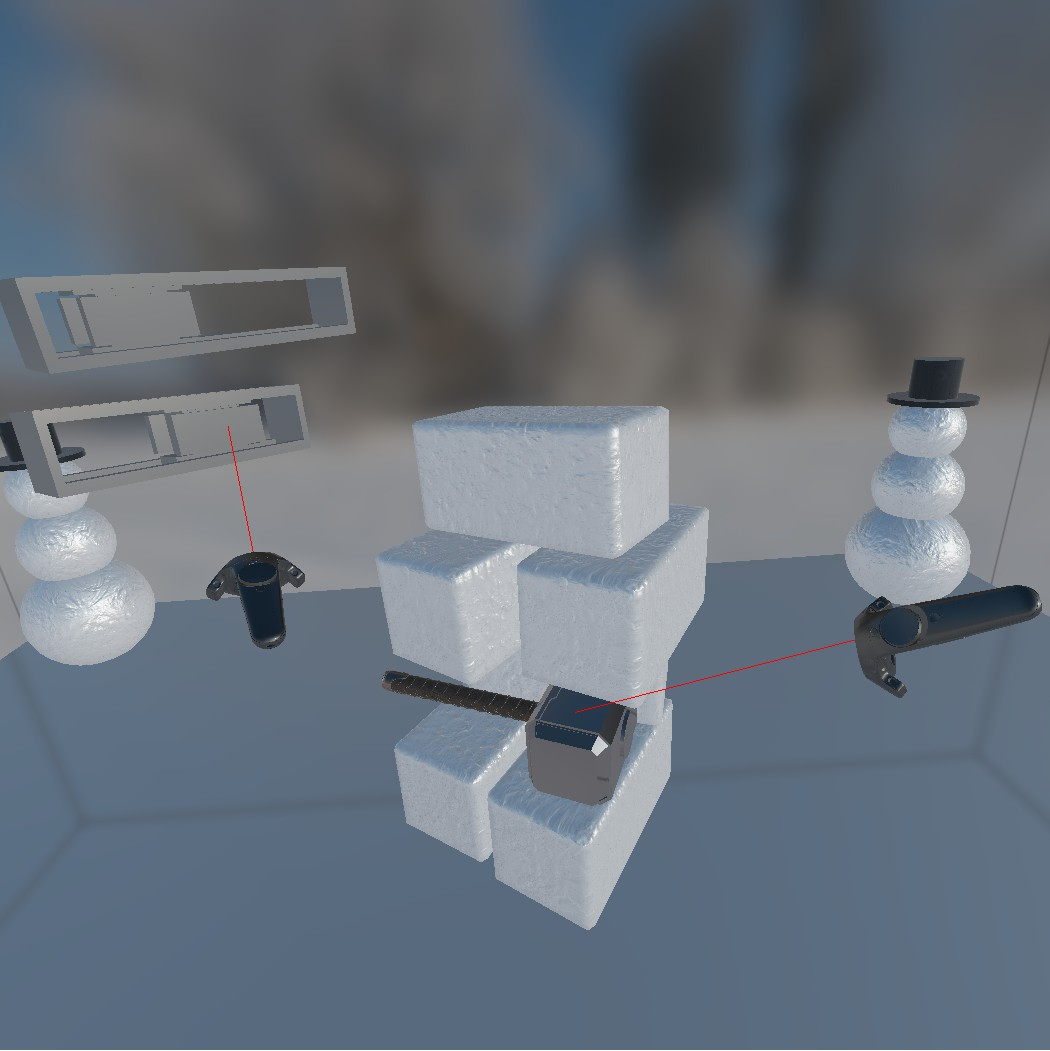
\includegraphics[width=0.8\linewidth]{screenshots/physics_a.jpg}
        \caption{Stacking}
    \end{subfigure}
    \begin{subfigure}{\linewidth}
        \centering
        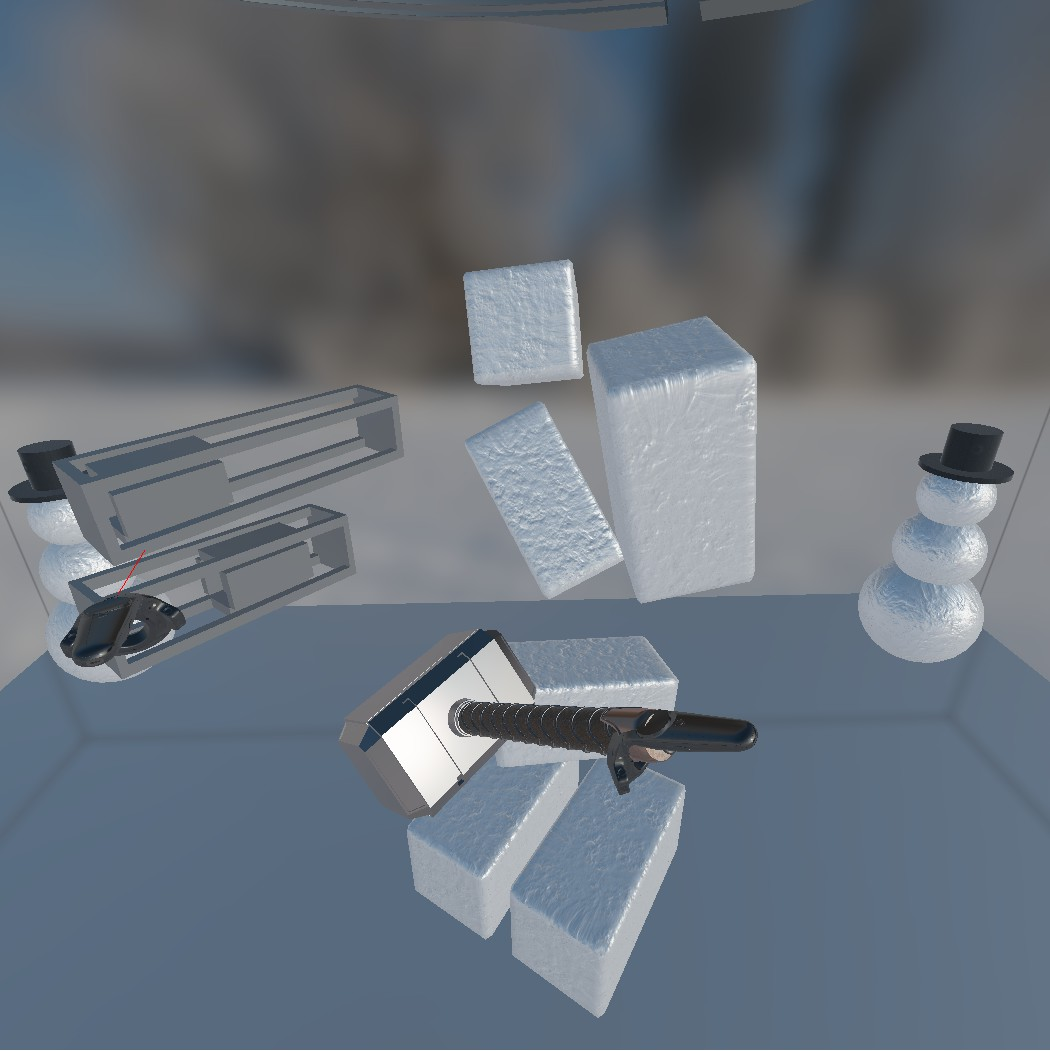
\includegraphics[width=0.8\linewidth]{screenshots/physics_b.jpg}
        \caption{Mjolnir Hitting Snowblocks}
    \end{subfigure}
    \caption{Physics Between Snowblocks and Mjolnir}
    \label{fig:physics}
\end{figure}

\subsection{Global User Interface}

For our project we also created a module which allowed the user to turn on and
off \textit{Let's Get Physical} and \textit{Snowflakes}. This module rendered
two boxes, each of which toggles on and off one of the applications. We stored
some minimal state about whether or not each application is enabled. If the
application is not enabled, its functions are not called and thus, since we are
using immediate mode, the objects are not rendered. When the application is
toggled back on, the functions for that application begin to be called again and
the objects associated with that application are rendered again. This toggle
functionality is shown in Figure~\ref{fig:toggles}.

\begin{figure}[H]
    \begin{subfigure}{\linewidth}
        \centering
        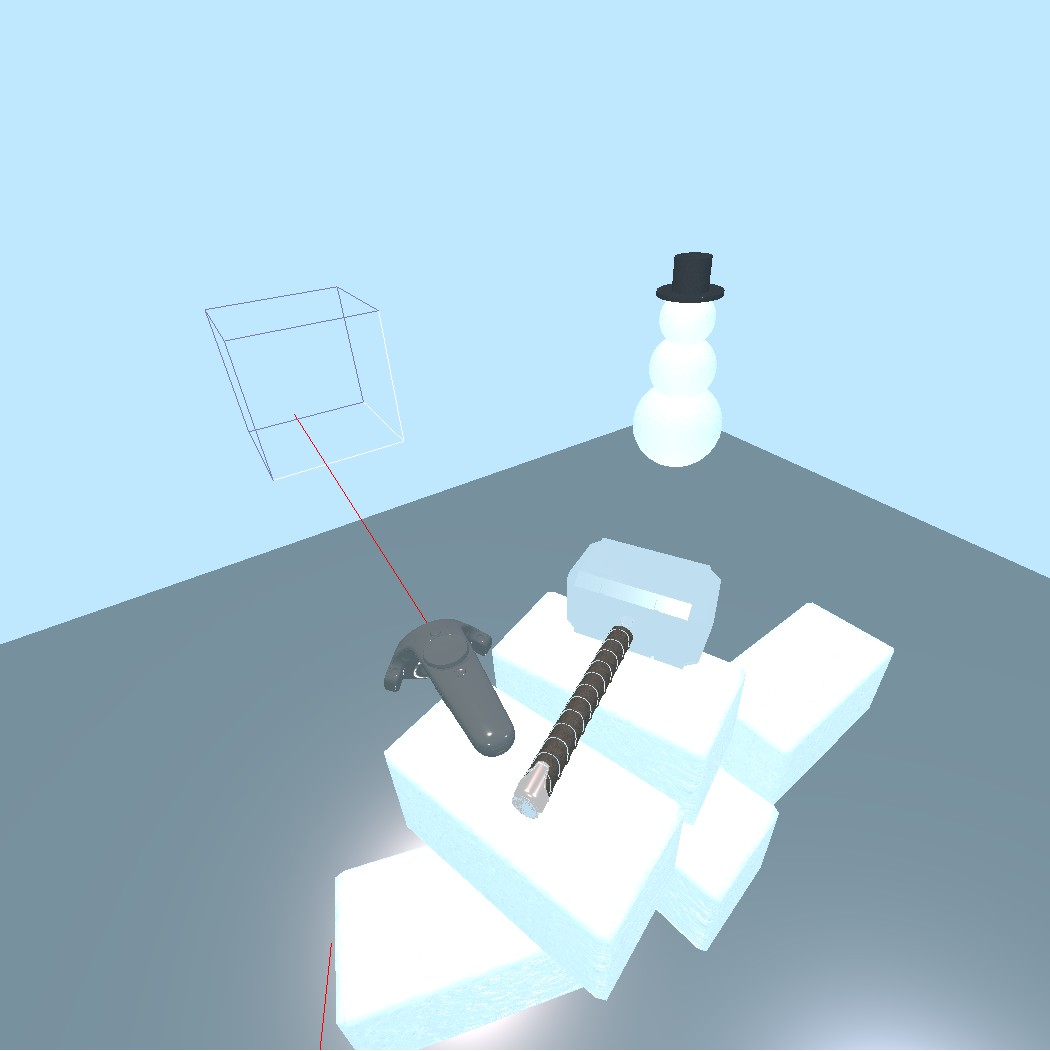
\includegraphics[width=0.8\linewidth]{screenshots/toggle_a.jpg}
        \caption{Before}
    \end{subfigure}
    \begin{subfigure}{\linewidth}
        \centering
        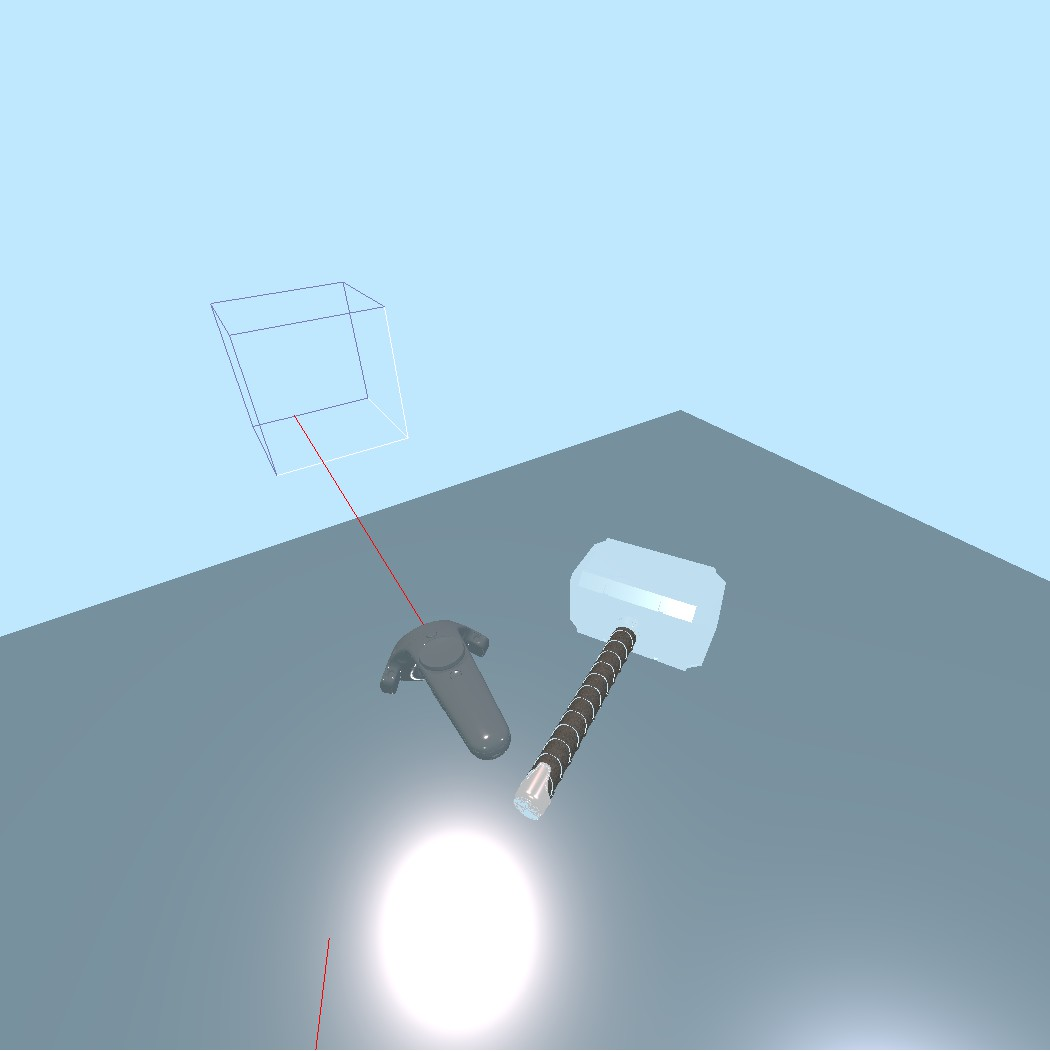
\includegraphics[width=0.8\linewidth]{screenshots/toggle_b.jpg}
        \caption{After}
    \end{subfigure}
    \caption{Application Toggles}\label{fig:toggles}
\end{figure}

This example illustrates the power of immediate mode. We did not have to go
through the entire scene removing or adding all of the elements associated with
the toggled application, we merely had to check a boolean value to determine
whether or not to call each applications' functions.

\subsection{Control Elements}

\texttt{flight-ui} includes a few control UI elements, notably a one-dimensional
slider. This slider component can be grabbed, moved, manipulated, and yanked.
Because all UI components use the immediate mode architecture, they are easily
associated with state information, simulation parameters, and even other
interface elements.

\begin{figure}[H]
    \begin{subfigure}{\linewidth}
        \centering
        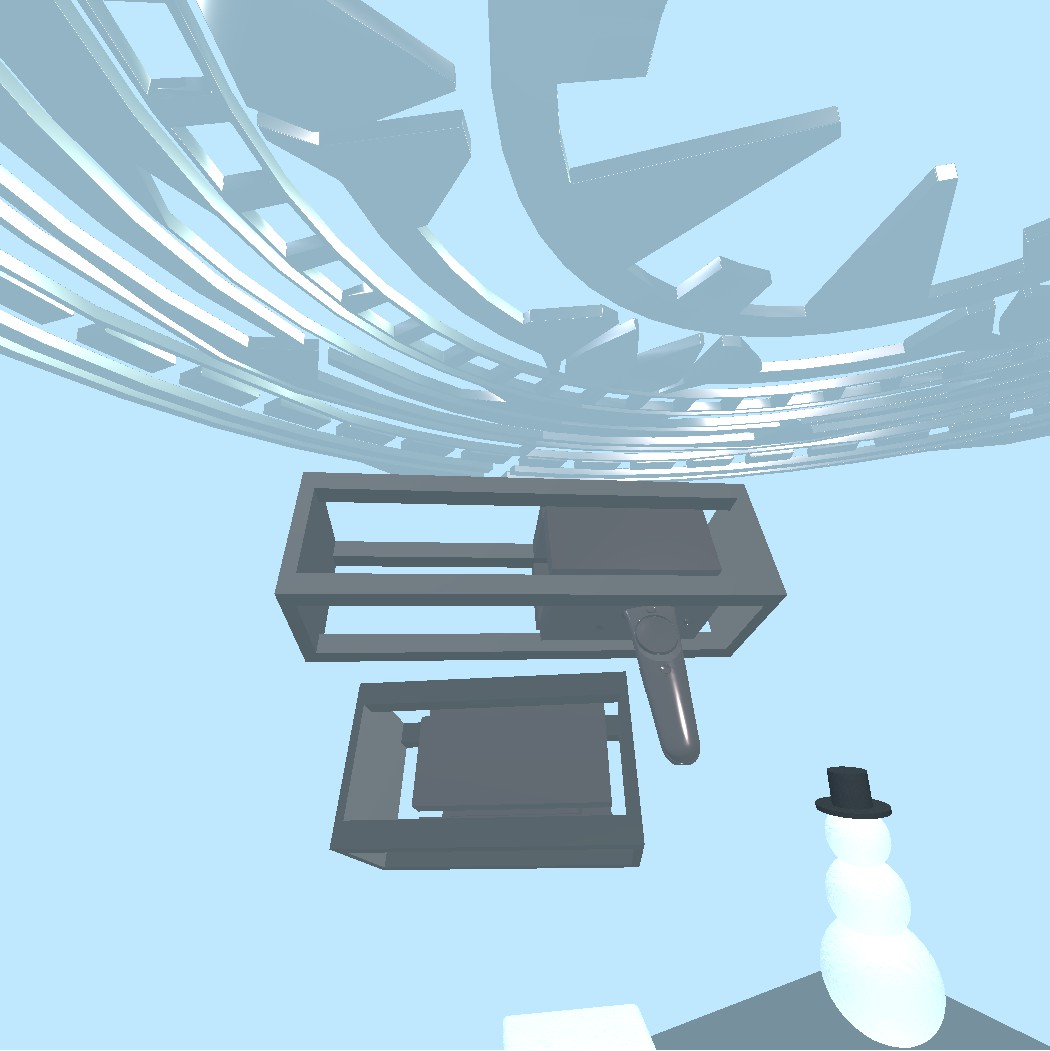
\includegraphics[width=0.8\linewidth]{screenshots/slider_a.jpg}
        \caption{Before}
    \end{subfigure}
    \begin{subfigure}{\linewidth}
        \centering
        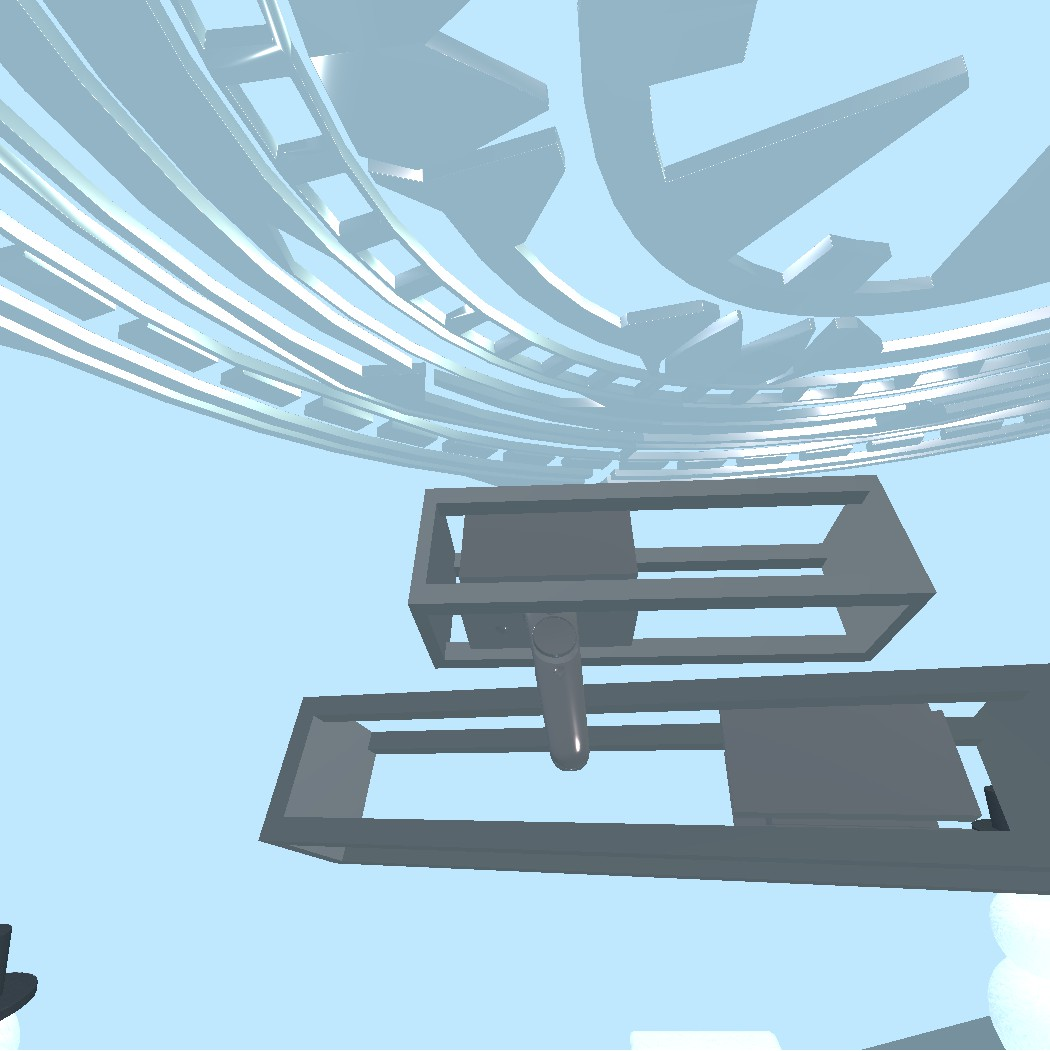
\includegraphics[width=0.8\linewidth]{screenshots/slider_b.jpg}
        \caption{After}
    \end{subfigure}
    \caption{Interdependent Sliders}
    \label{fig:sliders}
\end{figure}

Two slider elements are shown in Figure \ref{fig:sliders}. The first controls
the speed of the physics simulation and the second controls the length of the
first. This kind of interdependence is frustrating and bug-prone in a retained
mode system, but was a trival feature to add to our application.

\subsection{State Saving}

We also implemented the ability to save the state of the application. Each
module of the application individually defines a serialize and deserialize
function which converts the module state to a JSON format. When the user exits
and reopens the application, the state of the application is restored. By using
immediate mode, we are able to minimize the amount of state that we have to
store; we only need to store enough state to begin calling the same functions
once the application is reopened.
im
In the example of \textit{Snowflakes} we only need to store the location and
rotation of each snow block. Likewise for \textit{Let's Get Physical}; we only
need to store the location and rotation of Mjolnir.

\section{Conclusion}\label{sec:conclusion}

Over the past three months, we have explored a variety of user interface
implementations for virtual reality. While doing so, we have significantly
improved our knowledge of the Rust language and ecosystem, becoming familiar
with virtual reality tools and libraries. Additionally, we have developed,
almost from scratch, our own toolkit called Flight which takes a novel approach
to user interface and virtual reality application architecture.

Finally, as a demonstration of what we have learned through this independent
study, we created a variety of virtual reality environments and combined them
into one cohesive project.

We are excited to improve on the deferred immediate mode approach and
revolutionize the way people interact with computers.

{\printbibliography}

\end{document}
